\documentclass[aspectratio=169]{beamer} % Widescreen


% \usetheme{Madrid} % Clean theme, good for technical slides
\usetheme[progressbar=frametitle]{metropolis}

\usepackage{fontspec}
\setmainfont{Fira Sans}
\setsansfont{Fira Sans}

\definecolor{mycolor}{HTML}{1F77B4} % Custom blue accent
\setbeamercolor{alerted text}{fg=mycolor}
\setbeamercolor{structure}{fg=mycolor}

\title[Git Pro]{Git Pro: Beginners Guide to Git and GitHub}
\author{Sayan Ghosh}
\institute{IC\&SR, IIT Madras}
\date{\today}

\begin{document}

%----------------------------------
\begin{frame}
  \titlepage
\end{frame}

%----------------------------------
\begin{frame}{Agenda}
  \begin{itemize}
    \item Core Git Concepts
    \item GitHub Integration
    \item Branching \& Merging
    \item Collaboration: Pull Requests
    \item Automation with GitHub Actions
    \item Makefiles for Automation
    \item Command Line Essentials
    \item Real-World Workflow
    \item Wrap-up \& Q\&A
  \end{itemize}
\end{frame}

%----------------------------------
\section{Introduction}

\begin{frame}{Why Version Control?}
  \begin{itemize}
    \item Keep track of changes in your work
    \item Collaborate safely without overwriting each other’s files
    \item Example: Version chaos vs Git timeline
  \end{itemize}
\end{frame}

%----------------------------------
\section{Core Git Concepts}

\begin{frame}{What is Git? What is GitHub?}
  \begin{itemize}
    \item Git: Local version control system
    \item GitHub: Remote hosting and collaboration
  \end{itemize}
\end{frame}

\begin{frame}{Key Concepts}
  \begin{itemize}
    \item Repository, Working Directory, Staging Area
    \item Commits \& History
  \end{itemize}
\end{frame}

\begin{frame}{Three Stages of Git}
  \begin{figure}
    \centering
    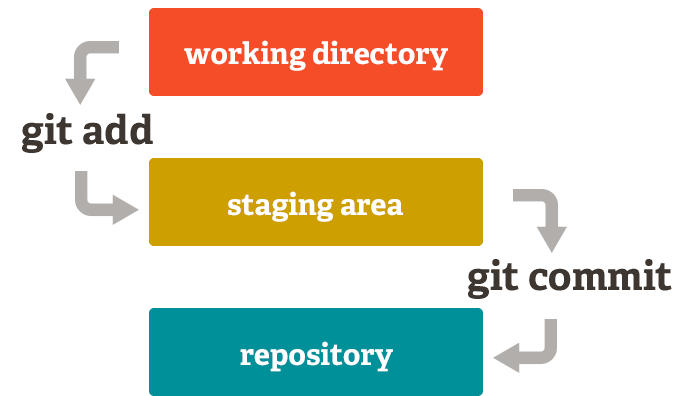
\includegraphics[width=0.8\textwidth]{res/stages.png}
    \caption{Three Stages of Git}
  \end{figure}
\end{frame}

\begin{frame}{Essential Commands}
  \begin{itemize}
    \item \texttt{git init}, \texttt{git add}, \texttt{git commit}
    \item \texttt{git status}, \texttt{git log}
  \end{itemize}
\end{frame}

%----------------------------------
\section{GitHub Integration}

\begin{frame}{Local to Remote}
  \begin{itemize}
    \item Add remote: \texttt{git remote add origin}
    \item Push changes: \texttt{git push}
    \item Clone: \texttt{git clone}
  \end{itemize}
\end{frame}

\begin{frame}{Demo: Connect Local Repo}
  \begin{enumerate}
    \item Create repo on GitHub
    \item Link remote
    \item Push first commit
  \end{enumerate}
\end{frame}

%----------------------------------
\section{Branching and Merging}

\begin{frame}{Why Use Branches?}
  \begin{itemize}
    \item Work on new features safely
    \item Resolve conflicts systematically
    \item Keep track of different development lines
  \end{itemize}
\end{frame}

\begin{frame}{Branches Can Get Messy}
\begin{figure}
  \centering
  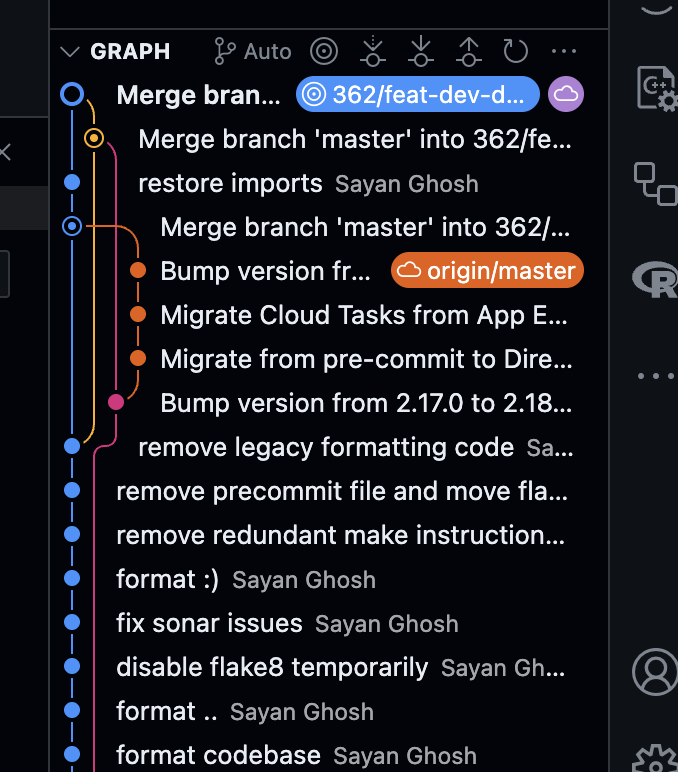
\includegraphics[width=0.4\textwidth]{res/branches.png}
  \caption{Branches can get messy!}
\end{figure}
\end{frame}

\begin{frame}{Basic Commands}
  \begin{itemize}
    \item \texttt{git branch}, \texttt{git checkout -b}
    \item \texttt{git merge}
    \item Resolving merge conflicts
  \end{itemize}
\end{frame}

%----------------------------------
\section{Collaboration}

\begin{frame}{Issues}
  \begin{itemize}
    \item Track bugs, feature requests
    \item Assign to team members
    \item Link issues to commits
  \end{itemize}
\end{frame}

\begin{frame}{Pull Requests}
  \begin{itemize}
    \item Review and discuss code before merging
    \item Assign reviewers, track changes
  \end{itemize}
\end{frame}

\begin{frame}{Git Flow vs GitHub Flow}
  \begin{itemize}
    \item Git Flow: Develop, feature, release, hotfix branches
    \item GitHub Flow: Simple, single main branch with feature branches
  \end{itemize}
\end{frame}

\begin{frame}{Interactive Group Task: GitHub Collaboration}

\begin{enumerate}
  \item Form groups of 3--4 members.
  \item One member creates a new GitHub repository for the group.
  \item Add all teammates as collaborators with \texttt{Write} access.
  \item Clone the shared repo to your local machine.
  \item Create issues for features to add.
  \item Create branches referring to the issues.
  \item Add or edit files.
  \item Push your branch and open a Pull Request (PR).
  \item Review each other's PRs and merge them.
  \item Intentionally create and resolve at least one merge conflict.
\end{enumerate}

\textbf{Tips:} Use clear commit messages, meaningful branch names, and communicate with your team!
\end{frame}

%----------------------------------
\section{Automation}

\begin{frame}{Intro to CI/CD}
  \begin{itemize}
    \item Continuous Integration \& Continuous Deployment
    \item Automate testing, linting, deployment
  \end{itemize}
\end{frame}

\begin{frame}{GitHub Actions}
  \begin{itemize}
    \item Workflows defined in YAML
    \item Trigger on push/pull request
    \item Example: Auto lint on push
  \end{itemize}
\end{frame}

%----------------------------------
\section{Makefiles}

\begin{frame}{Why Makefiles?}
  \begin{itemize}
    \item Automate repeated tasks: build, test, clean
    \item Simple syntax: \texttt{target: dependencies}
  \end{itemize}
\end{frame}

\begin{frame}{Makefiles with GitHub Actions}
  \begin{itemize}
    \item Call Makefile tasks in your workflow
    \item Example: \texttt{make test}
  \end{itemize}
\end{frame}

%----------------------------------
\section{Command Line Essentials}

\begin{frame}{Linux Commands}
  \begin{itemize}
    \item \texttt{ls}, \texttt{cd}, \texttt{cat}, \texttt{grep}, \texttt{chmod}
    \item Helpful for day-to-day developer tasks
  \end{itemize}
\end{frame}

%----------------------------------
\section{Putting It All Together}

\begin{frame}{Real-World Scenario}
  \begin{enumerate}
    \item Clone repo → branch → commit → PR → review → merge
    \item CI/CD runs automatically
  \end{enumerate}
\end{frame}

%----------------------------------
\section{Wrap-up}

\begin{frame}{Key Takeaways}
  \begin{itemize}
    \item Git for version control
    \item GitHub for collaboration
    \item Automate with Actions and Makefiles
  \end{itemize}
\end{frame}

\begin{frame}{Resources}
  \begin{itemize}
    \item GitHub Learning Lab
    \item Official docs and cheat sheets
    \item Practice on real projects!
  \end{itemize}
\end{frame}

\begin{frame}{URL Submission \& Feedback}
  \begin{itemize}
    \item Submit your GitHub repo URL and your feedback for this workshop.
    \item Use the form: \url{https://forms.gle/my9gXm8ETkcqy9Up9}
    \item or scan the QR Code:
  \end{itemize}

  \begin{figure}
    \centering
    
\includegraphics[width=0.3\textwidth]{res/feedback.png}
    \caption{Scan to submit your URL and feedback!}
  \end{figure}
\end{frame}

\begin{frame}{Thank You!}
  \begin{center}
    Questions? \\
    Contact: sayan@study.iitm.ac.in
  \end{center}
\end{frame}

\end{document}
